% small.tex
\documentclass[t]{beamer}
\usepackage{graphicx}
\usetheme[hideothersubsections]{Goettingen}
\setbeamercolor{palette primary}{bg=structure.fg!25}
\setbeamercolor{palette secondary}{bg=structure.fg!10,fg=black}
\useinnertheme{rectangles} 
\useoutertheme{infolines} 
\author[TAES]{Thomas Smith} 
\title[CM30174/CM50206]{CM30174 + CM50206\\Intelligent Agents}
\institute[Bath/CS]{East Building}
\date{December 8, 2013} 
\begin{document}


%--- the titlepage frame -------------------------%
\begin{frame}
  \titlepage
\end{frame}

%--- the presentation begins here ----------------%
\section{Overview}
\subsection{Paper Overview}
\begin{frame}[c]{Paper Overview}
	\begin{quote}
		``Towards an environment interface standard for agent platforms''
	\end{quote}
	\hfill Tristan M. Behrens, Koen V. Hindriks, J{\"u}rgen Dix\\
	\hfill {\tiny \textit{Annals of Mathematics and Artificial Intelligence} (2011), 61:261--295.}
\end{frame}
\subsection{Problem Overview}
\begin{frame}{Problem Overview}
	Issues:
	\begin{itemize}
		% \pause
		\item There are many Agent Programming Languages (\emph{APL}s)
		% \pause
		% \begin{columns}
		% 	\column{.4\textwidth}
		% 		\begin{itemize}
		% 			\item \textsc{Jadex}
		% 			\item GOAL
		% 		\end{itemize}
		% 	\column{.4\textwidth}
		% 		\begin{itemize}
		% 			\item \textit{Jason}
		% 			\item 2APL
		% 		\end{itemize}
		% \end{columns}
		\begin{itemize}
			\item 2APL
			\item \textsc{Goal}
			\item \textsc{Jadex}
			\item \textit{Jason}
		\end{itemize}
		% \pause
		\item Multiple Environments
		% \pause
		\begin{itemize}
			\item Agent Competitions
			\item Unreal Tournament 2004
		\end{itemize}
		% \pause
		\item How can we connect / compare these components?
		% \pause
		\begin{itemize}
			\item Connections: TCP/IP, RMI, wrapping Java code, JNI
			% \pause
			\item Comparisons: we can't.
		\end{itemize}
	\end{itemize}
\end{frame}

\subsection{Goals}
\begin{frame}{Goals}
		%Motivation
	\begin{itemize}
		\item Implementing an environment interface standard would:\nolinebreak\begin{itemize}
			\item make already working environments widely available
			\item facilitate distribution of current and future environments
			\item allow direct comparison of APL platforms
			\item enable the develpment of a fully heterogeneous multi-agent system (\emph{MAS})
		\end{itemize}
		% \begin{quote}
		% 	Lessons learned have not been documented well enough to enable transfer of knowledge in this area
		% \end{quote}
		%Requirements
		\item In order to be accepted as a standard, it should:
		\begin{itemize}
			\item Provide an interface that is as \textit{generic as possible}
			\item \textit{Reuse as much as possible} from existing interfaces
			%obvious trade-off here
		\end{itemize}
		\item Therefore the objective is to: 
		\begin{itemize}
			\item[] ``\textit{Design and develop an environment interface standard (\emph{EIS}) that facilitates connecting agents programmed in various agent platforms to environments.}''
		\end{itemize}
	\end{itemize}
\end{frame}
\begin{frame}{Goals (contd.)}
	\begin{itemize}
		\item No assumptions need to be made about the internal structure or behaviour of any of the environments or entities
		\item However, the agent platform needs to support a minimal agent-based abstraction: \linebreak \textit{Actions and percepts are treated as first-class entities.}
		\item The standard is based on:
		\begin{itemize}
			\item A meta-model for agent-environment interaction
			\item A set of principles that encode useful constraints for implementing the standard
		\end{itemize}
		\item The meta-model arises from a study of existing APLs, and avoids restricting existing approaches
		\item The princples are based on the requirements of the project, and observed best practices among existing work
	\end{itemize}
\end{frame}
\begin{frame}{Principles}
	\begin{enumerate}
		\item \textit{Portability}: .jar files are suggested but not required, for easy exchange of environments between platforms
		\item \textit{Generality}: The \emph{EIS} should impose minimal restrictions on the platform or environments. Assumptions about the agents or the environments should be avoided
		\item \textit{Separation of concerns}: Agents are \textit{separated} from the environment
		\item \textit{Unified connections}: The \emph{EIS} should facilitate communications between agents and the environment(s)
		\item \textit{Standards for actions/percepts/events/etc.}: The \emph{EIS} should provide a convention for communicataing about concepts, without restricting any existing approach
		\item \textit{Support for heterogeneity}: The interface standard needs to facilitate heterogeneity - connections between an environment and agents of multiple types
	\end{enumerate}
\end{frame}
\section{Existing Work}
\subsection{Related Work}
\begin{frame}{Related Work}
	There are a number of other projects that support generic connections between agents and an environment:
	\begin{itemize}
		\item A\&A: a generic paradigm for modeling environments. Implemented in the distributed middleware \textsc{CArtAgO}
		\item \textsc{Soar} is an architecture for knowledge-rich agents capable of intelligent behavior in dynamic environments
		\item GameBots and Pogamut are a pair of projects designed to allow agents to control bots in UT2004. A number of other projects use them as an initial base
		\begin{itemize}
			\item pyPOSH aims to use Behaviour Oriented Design agents
			\item the ACT-R cognitive architecture uses GameBots
		\end{itemize}
		\item The high level architecture (HLA) is a federated architecture for distributed simulations
		\item The \textit{UtJackInterface} defines another UT2004 interface from scratch - none of these approaches facilitate reuse
	\end{itemize}
	% does not facilitate reuse
\end{frame}
\subsection{Existing APLs}
\begin{frame}{Existing Agent Programming Languages}
	\begin{itemize}
		\item A number of existing APLs indicate common and uncommon features that the meta-model must support
		\begin{itemize}
		\item 2APL
		% Environments are distributed as jar-files. Agents can be associated with several environments, jars have to be in the user-directory. Agents are objects, there is a communications format
		\item \textsc{Goal}
		% Environments are distributed as jar-files. There is a scheduler.
		\item \textsc{Jadex}
		% Environments exist as belifs of the agents.
		\item \textit{Jason}
		% Environments are distributed as jar-files. Each MAS has at most one environment. Sophisticated abstract environments
		\end{itemize}
		\item Though each APL is designed to fulfil similar purposes, they vary in implementation details
		\begin{itemize}
			\item 2APL provides a common format for exchanging data between agents and the environment
			\item \textsc{Goal} uses a scheduler to manage execution of agents
			\item \textsc{Jadex} store environments as beliefs of the agents
			\item \textit{Jason} provides spohisticated abstract environments
		\end{itemize}
		\item The different APLs have differing degrees of environment management functionality available
	\end{itemize}
\end{frame}
\subsection{Existing Environments}
\begin{frame}{Existing Environments}
\end{frame}
\section{EIS}
\subsection{Meta-model}
\begin{frame}{Meta-model}
	\begin{figure}
		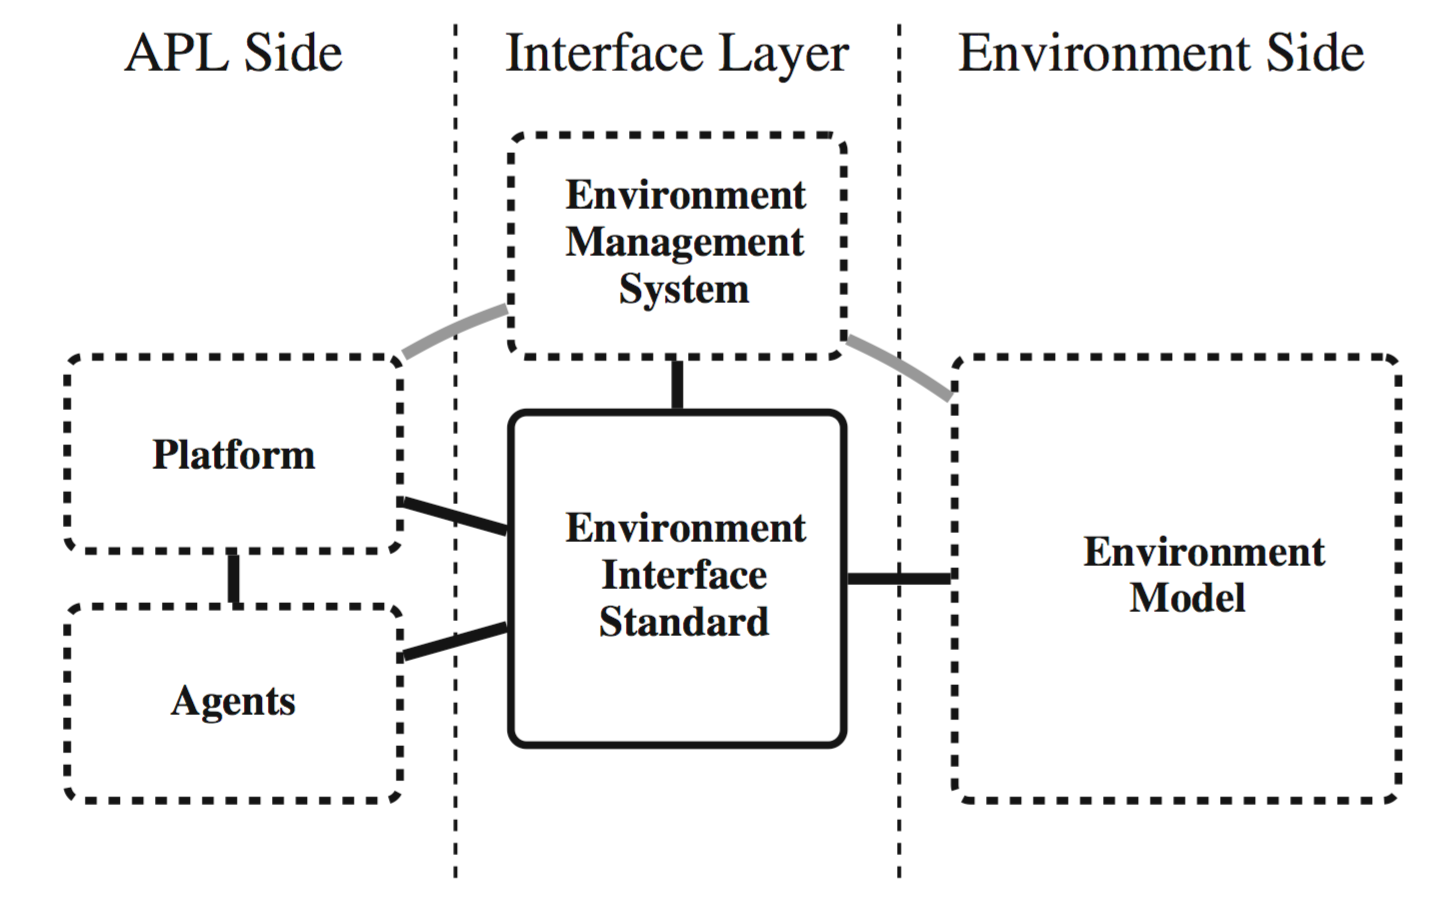
\includegraphics[width=0.6\linewidth]{metamodel}
	\end{figure}
% This model also includes generic functionality for managing an environment.
% The model introduced below is called a meta model as it does not describe a specific agent–environment interface but is intended to describe generic functionality that should be available in any agent-based interface supporting agent–environment interaction.
	\small
	\begin{enumerate}
		\item<1-> \textit{Agent}\only<1>{: able to perceive its environment through sensors and act upon that environment through effectors.}
		\item<2-> \textit{Environment model}\only<2>{: contains \textit{controllable entities} that give agents effective and sensory presence in the environment.}
		\item<3-> \textit{Platform}\only<3>{: instantiates and executes agents; connects agents to the environment and controllable entities.}
		\item<4-> \textit{Environment management system (EMS)}\only<4>{: provides actions for managing an environment, such as setup, pause and reset.}
		\item<5-> \textit{Environment interface standard (EIS)}\only<5>{: the layer that connects the platform, the EMS, and the agents to the environment(s).}
	\end{enumerate}
\end{frame}
\subsection{Interface Immediate Language}
\begin{frame}{Interface Immediate Language}
\end{frame}
\subsection{Implementation}
\begin{frame}{Implementation}
\end{frame}
\section{Case Studies}
\subsection{Case Study: Elevator}
\begin{frame}{Case Study: Elevator}
	\begin{figure}
		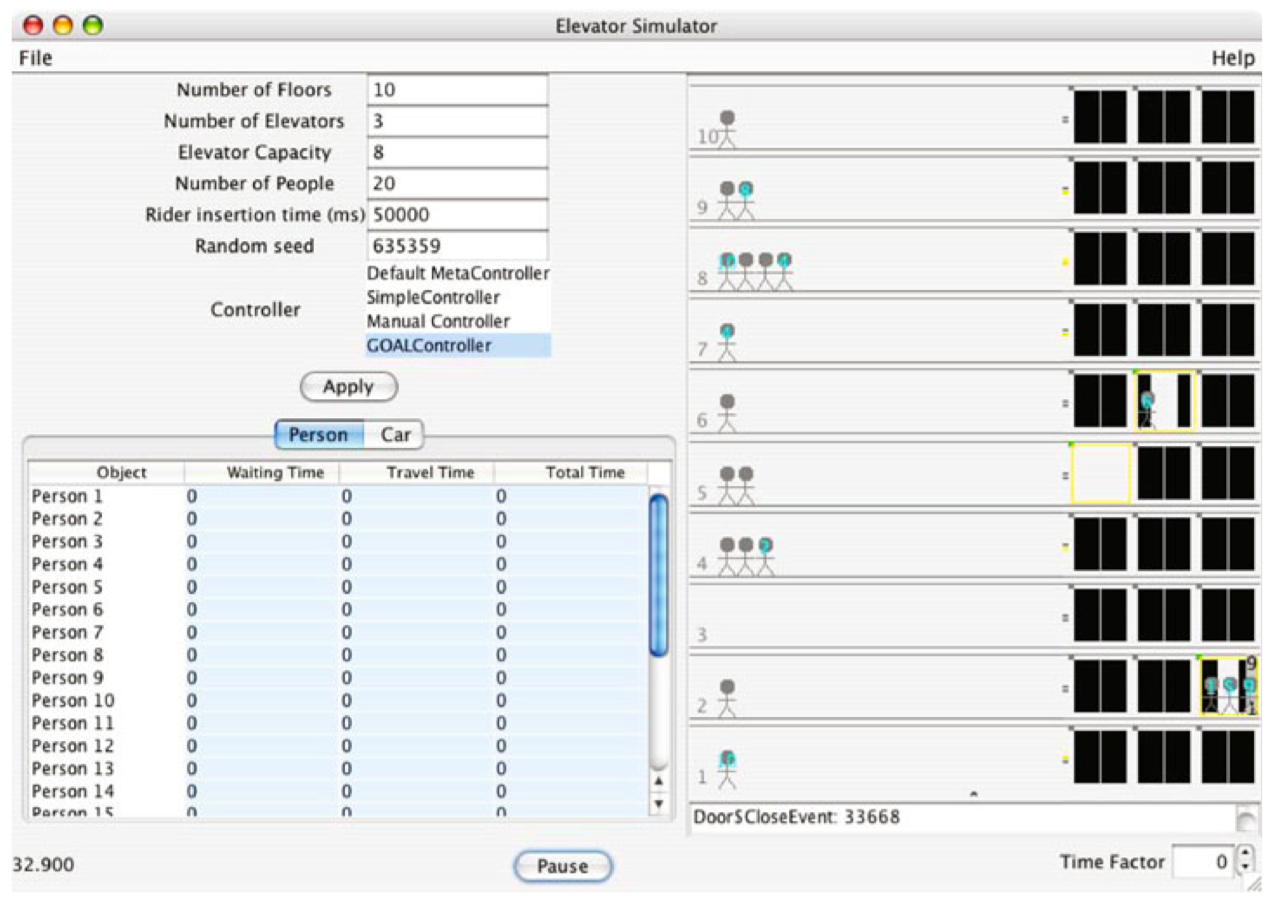
\includegraphics[width=0.6\linewidth]{elevator}
	\end{figure}
\end{frame}
\subsection{Case Study: Agent Contest}
\begin{frame}{Case Study: Agent Contest}
	\begin{figure}
		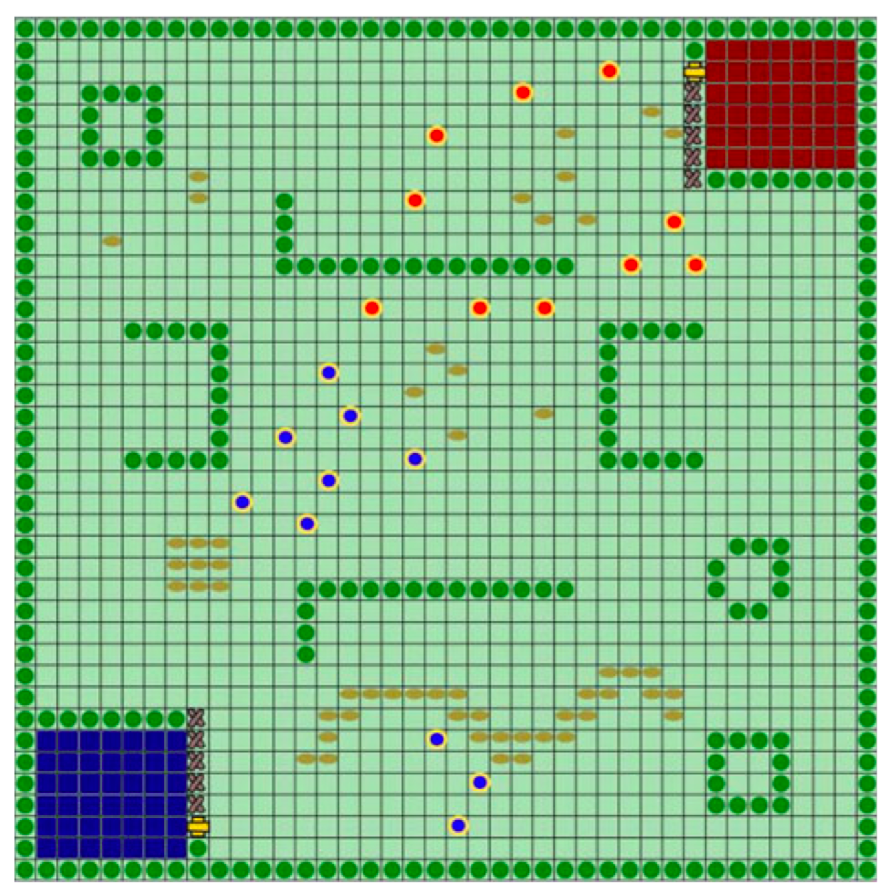
\includegraphics[width=0.6\linewidth]{cowboys}
	\end{figure}
\end{frame}
\subsection{Case Study: Unreal Tournament}
\begin{frame}{Case Study: Unreal Tournament}
	\begin{figure}
		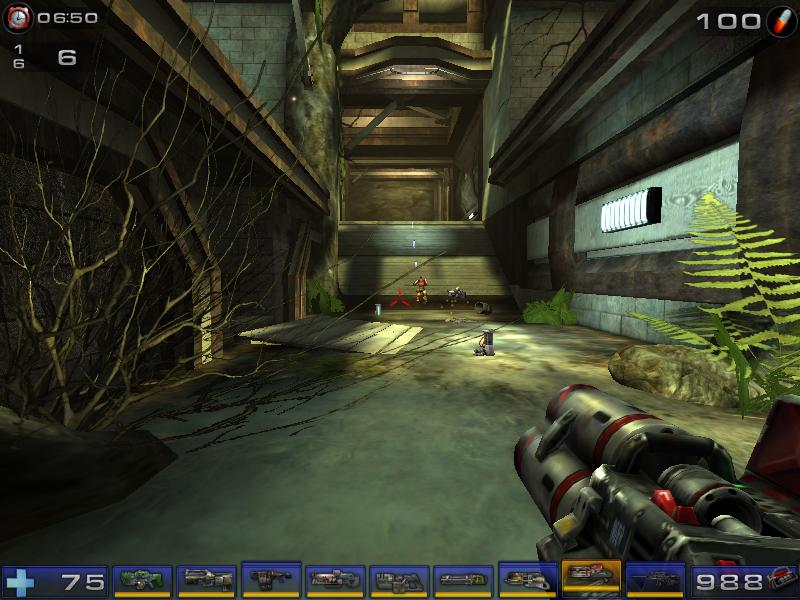
\includegraphics[width=0.6\linewidth]{ut2004}
	\end{figure}
\end{frame}
\section{Summary}
\begin{frame}{Summary}
	standard functionality is provided by the interface implementation itself
	agent platforms that support the interface can connect to any environment that implements the interface
\end{frame}
% \section{}
% \begin{frame}{Glossary}
% \end{frame}

\end{document}